\documentclass{article}
\usepackage[utf8]{inputenc}
\usepackage{mathtools,amssymb}
\usepackage{lipsum}
\usepackage{hyperref}
\usepackage{layout}
\usepackage{geometry}
\usepackage{listings}
\usepackage{booktabs}       % professional-quality tables
\usepackage{color}
\usepackage{pdfpages}
\usepackage{algorithm}
\usepackage{algpseudocode}
\usepackage{graphicx}
\graphicspath{{"../results/"}}
\newcommand*{\vertbar}[1][10ex]{\rule[-1ex]{0.5pt}{#1}}
\newcommand*{\horzbar}{\rule[.5ex]{2.5ex}{0.5pt}}
\newcommand{\norm}[2]{\left\lVert#1\right\rVert_#2}
\newcommand{\abs}[1]{\lvert#1\rvert}

\title{STATS370: Final Project}
\author{Erich Trieschman}
\date{2022 Fall Quarter}


\newcommand{\userMarginInMm}{10}
\geometry{
 left=20 mm,
 right=20 mm,
 top=20 mm,
 bottom=20 mm,
 footskip=5mm}

\newcommand*\circled[1]{\raisebox{.5pt}{\textcircled{\raisebox{-.9pt} {#1}}}}
\newcommand*\bspace{$\; \bullet \;$}

\hypersetup{
    colorlinks=true,
    linkcolor=blue,
    filecolor=magenta,      
    urlcolor=cyan,
    pdfpagemode=FullScreen,
}

\definecolor{dkgreen}{rgb}{0,0.6,0}
\definecolor{gray}{rgb}{0.5,0.5,0.5}
\definecolor{mauve}{rgb}{0.58,0,0.82}
    
\lstset{frame=tb, language=Python,
  aboveskip=3mm,
  belowskip=3mm,
  showstringspaces=false,
  columns=flexible,
  basicstyle={\small\ttfamily},
  numbers=none,
  numberstyle=\tiny\color{gray},
  keywordstyle=\color{blue},
  commentstyle=\color{dkgreen},
  stringstyle=\color{mauve},
  breaklines=true,
  breakatwhitespace=true,
  tabsize=3}

\begin{document}
\maketitle

% \tableofcontents

\section{Introduction}
In this project I am provided with a labeled dataset of gene expression measurements and I am asked study the the parameters that characterize their distribution. This problem assumes that gene expression measurements follow independent normal distributions, parameterized by the same, unknown, standard deviation, and different, unknown, means. I use Bayesian methods to study these parameters by evaluating the shape, central tendency, and variability of their posterior distribution using priors provided to me in the problem. A full characterization of the provided gene expression models and prior distributions, as well as the form of my target posterior distribution, is included in Appendix \ref{sec:a_post}. 

My parameter of interest, $\theta = (\sigma^2, \tau, \mu_1, \mu_2, \gamma_1, \gamma_2) \in \mathbb{R}^6$, is of high dimension. Calculating the posterior distribution, $p(\theta)$, directly, requires a six-dimensional integral. I choose instead to study statistics generated from samples from this posterior distribution. These I can draw using methods that only require computing a function, $f(\theta)$, that is proportional to the distribution of interest and much easier to compute. In asymptotics, studying statistics calculated from samples of this posterior distribution is analogous to studying the distribution itself.

I consider four sampling methods that enable me to draw samples from my target distribution: Metropolis-Hastings sampling, Gibbs sampling, Hamiltonian Monte Carlo sampling, and Importance sampling. In the sections that follow, I describe my implementation of these sampling methods, including the design choices I make for each, and then present my results from the sample posterior distribution. I conclude this project with a comparison of these techniques, taking into account each one's scalability.



%------------------------------------------------------------------------
% METROPOLIS HASTINGS
\section{Metropolis-Hasting}
\label{sec:MH}
\subsection{Implementation}
In this section I use the Methropolis-Hasting algorithm to generate samples from my posterior distribution of model parameters. At each step, this algorithm requires the choice of a candidate distribution, $q(\theta)$, from which to draw candiate samples, and accepts those samples according to an acceptance probability that is determined by the currently selected sample and the function proportional to my posterior distribution, $f(\theta)$.

I choose the candidate distribution at each step to match the support of the target parameter space. To facilitate implementation, I construct distributions with the same shape at each step, only shifted so that the mean of the candidate distribution is located at the current accepted sample point. In this way I can propose candidates with a higher likelihood of being accepted. To facilitate implementation, my candidate distribution is the composition of independent distributions for each parameter. 

In Table \ref{tab:mh_cand}, I describe the independent probability distributions used to construct my candidate distribution, assuming at step i that $\theta_i = (\sigma^2_i, \tau_i, \mu_i, \gamma_i)$. Note to generate candidate samples of $\sigma^2$ that lie in the right domain, I use a log-normal distribution. To properly implement this, I include the Jacobian of the transformation, as shown below.

\begin{align}
  q(\theta \mid \theta_i) &=  q(\sigma^2\mid\sigma^2_i) q(\tau\mid\tau_i)q(\mu\mid\mu_i)q(\gamma \mid \gamma_i), \textrm{ where }\\
  q(\sigma^2 \mid \sigma^2_i) &= \frac{1}{\sqrt{2\pi\nu_{\sigma^2}}}\exp\left[\frac{1}{2\nu_{\sigma^2}}\left(\log(\sigma^2) - \log(\sigma^2_i)\right)^2\right]\left| \frac{d}{d\sigma^2}\log(\sigma^2)\right|  
\end{align}

\begin{table}[H]
  \small
  \begin{center}
    \begin{tabular}{llc}
    \textbf{Parameter} & \textbf{Distribution} & \textbf{Support} \\
    \midrule
    $e^{\sigma^2_{i+1}}$ & $Norm(\mu=\log(\sigma^2_i), \sigma^2=\nu_{\sigma^2})$ & $(0, \infty)$\\
    $\tau_{i+1}$ & $TruncNorm(\mu=\tau_i, \sigma^2=\nu_{\tau}, lb=0, ub=1)$ & $[0, 1]$\\
    $\mu_{i+1}$ & $Norm(\mu=\mu_i, \Sigma=\nu_{\mu}I)$ & $(-\infty, \infty)$ \\
    $\gamma_{i+1}$ & $Norm(\mu=\gamma_i, \Sigma=\nu_{\gamma}I)$ & $(-\infty, \infty)$\\
    \bottomrule
    \end{tabular}
    \end{center}
    \caption{\label{tab:mh_cand} Form of candidate distribution, assuming independence across distributions}
\end{table}

In this algorithm I have ample flexibility to define my candidate distribution, $q(\theta)$. To tune this algorithm, my objective is to construct a candidate distribution that proposes candidates with high probability of being accepted. After all, the higher the acceptance rate, the more samples I can generate per iteration of the algorithm. 

Yet, naively constructing an effective candidate distribution can be difficult as such a distribution needs to propose samples that i) sufficiently explore the entire parameter space and ii) have a high enough probability of returning to the original sample. In my implementation of this algorithm, I notice a tradeoff between these requirements, where lower-variance distributions around the current sample points increase the acceptance probability, but also increase the autocorrelation between points. Reducing autocorrelation between sample points is important to reduce bias of the overall sample. I use a grid search to optimize this tradeoff by tuning the variance in each distribution above, $(\nu_{\sigma^2}, \nu_\tau, \nu_\mu, \nu_\gamma)$, noting in the literature that an optimal acceptance rate for this tradeoff is between 0.25 and 0.35 when the parameter space is greater than 4 dimensions \cite{Roberts}. Table \ref{tab:mh_gridsearch} in Appendix \ref{sec:a_mh} details the results of my tuning. 

In Algorithm \ref{alg:mh}, I present my implemented approach.

\begin{algorithm}[h]
  \caption{\label{alg:mh}Metropolis-Hastings algorithm}
    \begin{algorithmic}[1]
      \State $\theta_0 \longleftarrow$  Initialize
      \For{t=0, \dots, T}
        \State $\theta_{cand} \sim q(\theta) := q(\sigma^2\mid\sigma^2_t)q(\tau\mid\tau_t)q(\mu\mid\mu_t)q(\gamma \mid \gamma_t)$
        \State $a_t \longleftarrow \min\left(\frac{f(\theta_{cand})q(\theta_t\mid\theta_{cand})}{f(\theta_t)p(\theta_{cand}\mid\theta_t)}\right)$
        \State $u_t \sim Unif[0,1]$
        \If{$u_t \leq a_t$}
          \State $\theta_{t+1} \longleftarrow \theta_{cand}$
        \Else 
          \State $\theta_{t+1} \longleftarrow \theta_t$
        \EndIf
      \EndFor
    \end{algorithmic}
  \end{algorithm} 

\subsection{Results}
Below I present results from running the Metropolis-Hastings algorithm for $T=100,000$ iterations and hyperparameters, $\nu = (0.01, 0.01, 0.001)$. Figure \ref{fig:mh_dist} and Figure \ref{fig:mh_acorr} visualize the acceptance rate of each candidate sample point and the autocorrelation of each parameter -- these are the two the performance metrics used for the grid search described above. Figure \ref{fig:mh_marg} visualizes the sample points drawn from this algorithm at each step (left side), as well as their accumulated marginal distributions (right side). I also I present univariate statistics in Table \ref{tab:mh_univar} as well as the covariance between each parameter pair in Table \ref{tab:mh_covar}. 

I observe that the Metropolis Hastings algorithm yields a Markov Chain producing samples that have a clear mean and stable variance. I see this best in Figure \ref{fig:mh_marg}, where I observe the algorithm producing samples that explore the upper and lower limits of each parameter value, while also showing a clear central tendency. As expected, each parameter value lies within its domain. While I selected hyperparameters for this model to minimize autocorrelation, I do see that my samples for $\sigma^2$ still have a high autocorrelation (greater than 0.4 after 200 samples), especially relative to the other parameter values which have virtually no autocorrelation after about 50 samples. This could mean that the distribution for $\sigma^2$ is biased, although with such a large sample size this becomes less of a concern. 

\begin{figure}[H]
  \centering
  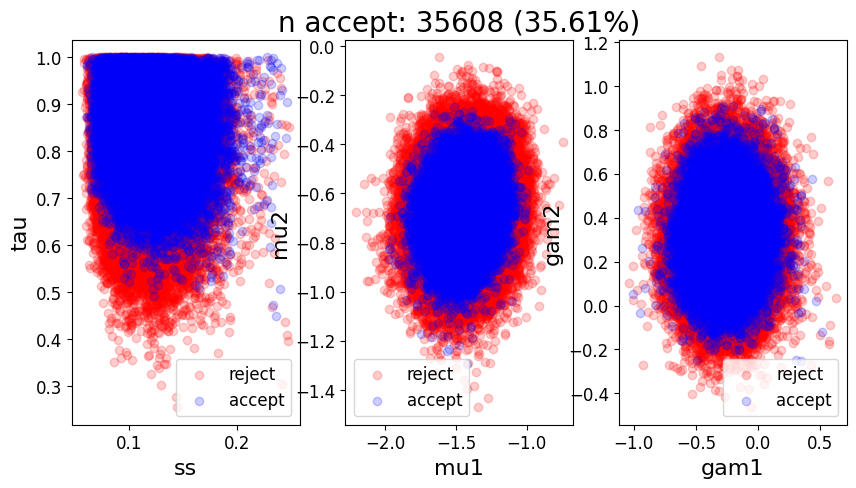
\includegraphics[width=.8\linewidth]{"./mh_dist.png"}
  \caption{\label{fig:mh_dist} Bivariate distributions for accepted and rejected candidate parameters drawn from Metropolis-Hastings}
\end{figure}

\begin{figure}[H]
  \centering
  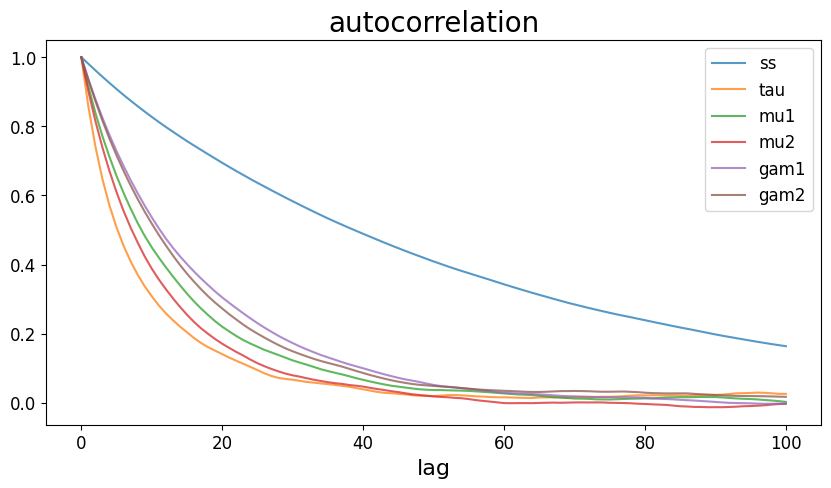
\includegraphics[width=.8\linewidth]{"./mh_acorr.png"}
  \caption{\label{fig:mh_acorr} Autocorrelation for each parameter drawn from Metropolis-Hastings}
\end{figure}

\begin{figure}[H]
  \centering
  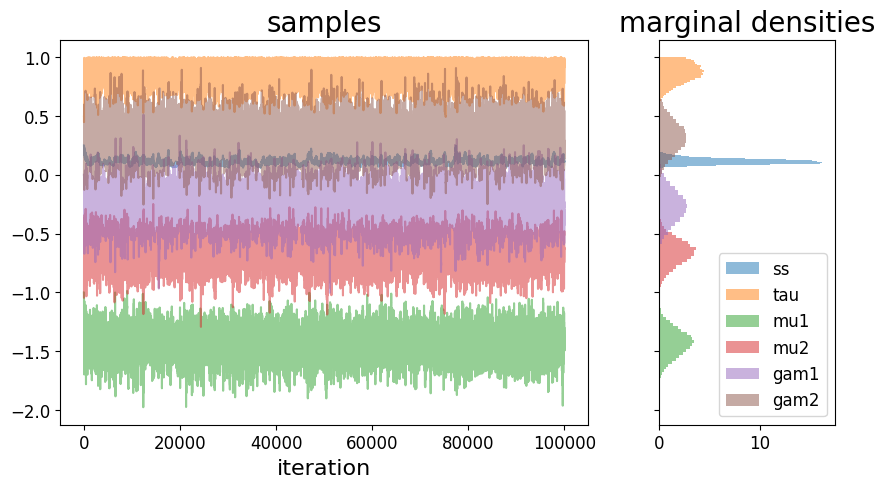
\includegraphics[width=.8\linewidth]{"./mh_marg.png"}
  \caption{\label{fig:mh_marg} Evolution of the Metropolis-Hastings sampling algorithm and accumulated marginal distributions}
\end{figure}

\begin{table}[H]
  \begin{center}
    \begin{tabular}{lrrrrrr}
      {} &$\sigma^2$ & $\tau$ & $\mu_1$ & $\mu_2$ & $\gamma_1$ & $\gamma_2$ \\
      \midrule
      mean   &  0.128855 &  0.856592 & -1.437832 & -0.660407 & -0.269792 &  0.316120 \\
      var    &  0.000854 &  0.007508 &  0.016422 &  0.013851 &  0.024934 &  0.023575 \\
      median &  0.124435 &  0.864481 & -1.432695 & -0.657491 & -0.270956 &  0.317396 \\
      p0     &  0.060584 &  0.389299 & -2.154638 & -1.326388 & -0.958255 & -0.361611 \\
      p10    &  0.095844 &  0.738386 & -1.602141 & -0.809834 & -0.470537 &  0.121178 \\
      p25    &  0.107768 &  0.798937 & -1.520030 & -0.735483 & -0.373689 &  0.214412 \\
      p50    &  0.124435 &  0.864481 & -1.432695 & -0.657491 & -0.270956 &  0.317396 \\
      p75    &  0.145736 &  0.924773 & -1.350404 & -0.580824 & -0.166230 &  0.418696 \\
      p90    &  0.167346 &  0.966222 & -1.279685 & -0.514553 & -0.070925 &  0.509682 \\
      p100   &  0.327578 &  0.999997 & -0.861472 & -0.172091 &  0.399618 &  0.980294 \\
      \bottomrule
      \end{tabular}
  \end{center}
  \caption{\label{tab:mh_univar} Univariate statistics from samples drawn from Metropolis-Hastings}
\end{table}

\begin{table}[H]
  \begin{center}
    \begin{tabular}{lrrrrrr}
      {} & $\sigma^2$ & $\tau$ & $\mu_1$ & $\mu_2$ & $\gamma_1$ & $\gamma_2$ \\
      \midrule
      $\sigma^2$   &  0.000854 & -0.000323 & -0.000197 & -0.000117 &  0.000087 & -0.000238 \\
      $\tau$  & -0.000323 &  0.007508 &  0.005160 &  0.003291 & -0.000687 &  0.000761 \\
      $\mu_1$  & -0.000197 &  0.005160 &  0.016422 &  0.002575 & -0.007119 &  0.000374 \\
      $\mu_2$  & -0.000117 &  0.003291 &  0.002575 &  0.013851 & -0.000793 & -0.005262 \\
      $\gamma_1$ &  0.000087 & -0.000687 & -0.007119 & -0.000793 &  0.024934 & -0.000133 \\
      $\gamma_2$ & -0.000238 &  0.000761 &  0.000374 & -0.005262 & -0.000133 &  0.023575 \\
      \bottomrule
      \end{tabular}
  \end{center}
  \caption{\label{tab:mh_covar} Covariance between parameters from distributions drawn from Metropolis Hastings}
\end{table}













% -------------------------------------------------------------------------------
% GIBBS
\section{Gibbs Sampling}
\subsection{Implementation}
In this section I use the Gibbs Sampling algorithm to generate samples from my posterior distribution of model parameters. Much like the Metropolis-Hastings algorithm, this approach generates candidate samples from a candidate distribution leveraging the properties of Markov Chains in such a way to ensure these samples follow my target distribution. 

Gibbs sampling is a strict improvement over the naive Metropolis-Hastings algorithm because the algorithm proposes candidates that are accepted at every step. A second advantage of this result is that the proposal candidates also explore the parameter space with very little autocorrelation because, by construction, the proposals are able to explore the entire parameter space. Therefore, Gibbs sampling is capable of maximizing both of the criteria (acceptance probability and autocorrelation) that I seek to tune in my naive Metropolis Hastings algorithm. As we prove in lecture, this success is accomplished because the candidate distributions are simply the target distribution of each parameter, conditional on the values of each other parameter. 

\begin{align}
  p(\theta[i] \mid Y, \theta[-i]) = \frac{p(\theta[i], \theta[-i] \mid Y)}{p(\theta[-i] | Y)} = f(\theta[i]) \propto p(\theta \mid Y) \textrm{ with fixed } \theta[-i], Y
\end{align}

The challenge presented by Gibbs Sampling is the need for a closed form probability distribution for each conditional target distribution. Fortunately, in this project I was able to derive these distributions, but in the general case such closed form distributions may not exist. I choose to implement the blocked version of Gibbs sampling for variables $\mu$ and $\gamma$ because of the simplicity of calculating their joint conditional distributions. I expect this to minorly improve the efficiency of my algorithm as this reduces the number of separate draws from conditional distributions I must make. I present my derivations of these calculations in Appendix \ref{sec:a_gibbs}. 

While the Gibbs sampling algorithm does not require hyperparameter tuning, it does require that I determine the order in which I scan and update the candidate parameter values. The two most common approaches are i) a systematic scan of the variables in the same order in each algorithm step and ii) a random (without replacement) scan of the variables in each algorithm step. I choose the latter approach, although I note that both approaches yield very similar results. I present my implemented Gibbs sampling approach using random scan in Algorithm \ref{alg:gibbs}. 

\begin{algorithm}[H]
  \caption{\label{alg:gibbs}Gibbs sampling algorithm}
    \begin{algorithmic}[1]
      \State $\theta_0 \longleftarrow$  Initialize
      \For{t=0, \dots, T}
        \State $idx \longleftarrow$ Shuffle($0,1,2,3$) \Comment{Randomize index order, only 4 indices because of my block approach}
        \State $\theta_{cand} \longrightarrow \theta_t$
        \For{i in {$idx$}} \Comment{$\theta[i]$ denotes $\theta$'s $i$'th component}
          \State $\theta_{cand}[i] \sim p(\theta[i] \mid Y, \theta_{cand}[-i])$ \Comment{$\theta[-i]$ denotes the vector excluding the $i$'th component}
        \EndFor
        \State $\theta_{t+1} \longleftarrow \theta_{cand}$
      \EndFor
    \end{algorithmic}
  \end{algorithm}


\subsection{Results}
Below I present results from running the Gibbs Sampling algorithm for $T=100,000$ iterations. Figure \ref{fig:mh_dist} and Figure \ref{fig:mh_acorr} visualize the joint distributions of samples, and the autocorrelation. Figure \ref{fig:mh_marg} visualizes the sample points drawn from this algorithm at each step (left side), as well as their accumulated marginal distributions (right side). I also present univariate statistics in Table \ref{tab:gibbs_univar} as well as the covariance between each parameter pair in Table \ref{tab:gibbs_covar}. 

As I expect, I observe that the Gibbs Sampling approach performs well, and outperforms the Metropolis Hastings algorithm. I observe that samples drawn in this method yields a Markov Chain producing samples that have a clear mean and stable variance. I see this best in Figure \ref{fig:mh_marg}, where I observe the algorithm producing samples that explore the upper and lower limits of each parameter value, while also showing a clear central tendency. As expected, each parameter value lies within its domain, and furthermore, I see minimal-to-no autocorrelation across all of my parameter values, addressing a minor concern presented in my Metropolis-Hastings algorithm.

\begin{figure}[H]
  \centering
  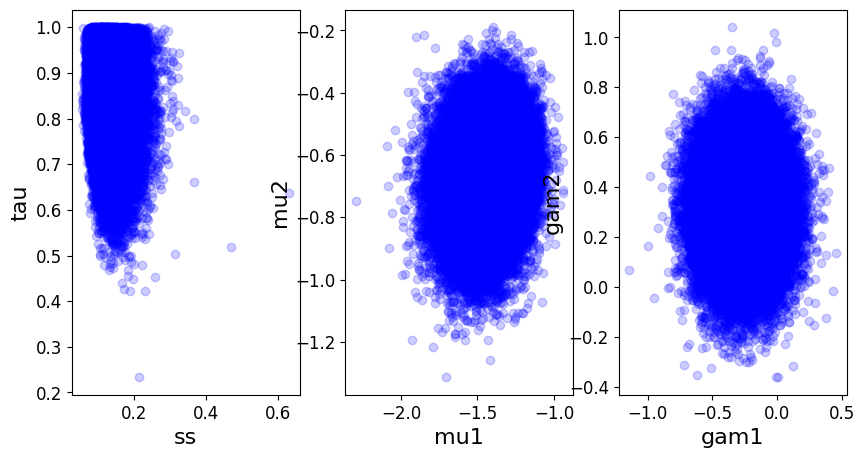
\includegraphics[width=.8\linewidth]{"./gibbs_dist.png"}
  \caption{\label{fig:gibbs_dist} Bivariate distributions for samples drawn from Gibbs sampling}
\end{figure}

\begin{figure}[H]
  \centering
  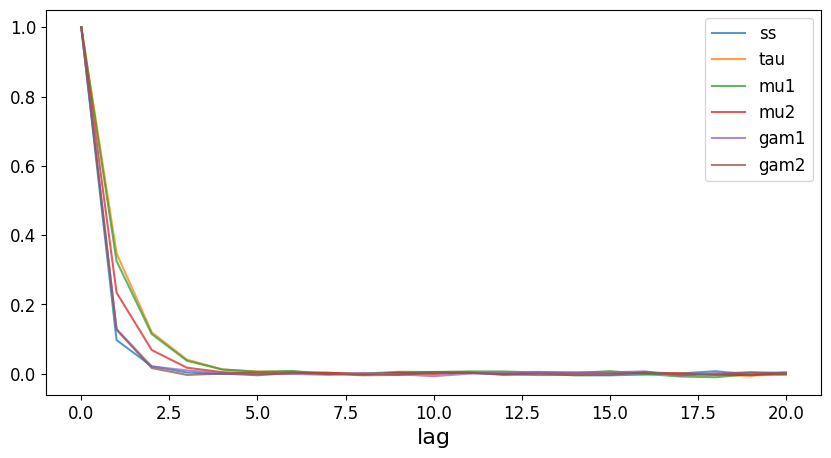
\includegraphics[width=.8\linewidth]{"./gibbs_acorr.png"}
  \caption{\label{fig:gibbs_acorr} Autocorrelation for each parameter value drawn from Gibbs sampling}
\end{figure}

\begin{figure}[H]
  \centering
  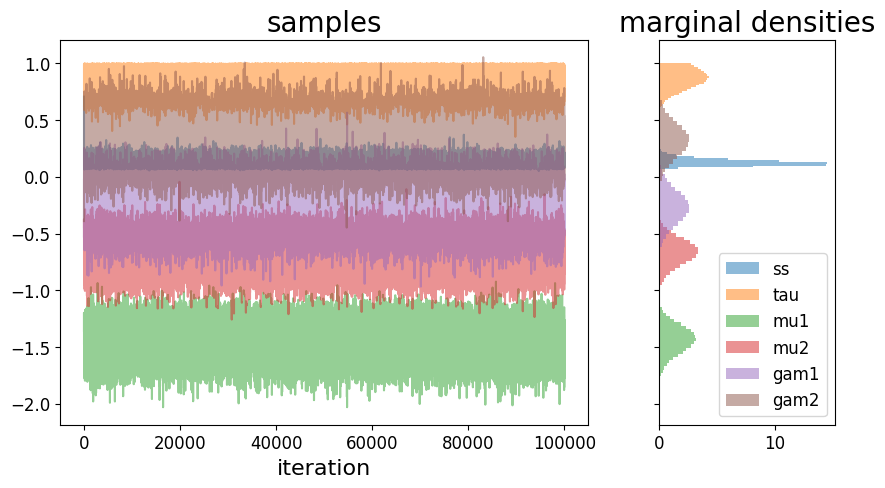
\includegraphics[width=.8\linewidth]{"./gibbs_marg.png"}
  \caption{\label{fig:gibbs_marg} Evolution of the Gibbs sampling algorithm and accumulated marginal distributions}
\end{figure}

\begin{table}[H]
  \begin{center}
    \begin{tabular}{lrrrrrr}
      &$\sigma^2$ & $\tau$ & $\mu_1$ & $\mu_2$ & $\gamma_1$ & $\gamma_2$ \\
      \midrule
      mean   &  0.128855 &  0.856592 & -1.437832 & -0.660407 & -0.269792 &  0.316120 \\
      var    &  0.000854 &  0.007508 &  0.016422 &  0.013851 &  0.024934 &  0.023575 \\
      median &  0.124435 &  0.864481 & -1.432695 & -0.657491 & -0.270956 &  0.317396 \\
      p0     &  0.060584 &  0.389299 & -2.154638 & -1.326388 & -0.958255 & -0.361611 \\
      p10    &  0.095844 &  0.738386 & -1.602141 & -0.809834 & -0.470537 &  0.121178 \\
      p25    &  0.107768 &  0.798937 & -1.520030 & -0.735483 & -0.373689 &  0.214412 \\
      p50    &  0.124435 &  0.864481 & -1.432695 & -0.657491 & -0.270956 &  0.317396 \\
      p75    &  0.145736 &  0.924773 & -1.350404 & -0.580824 & -0.166230 &  0.418696 \\
      p90    &  0.167346 &  0.966222 & -1.279685 & -0.514553 & -0.070925 &  0.509682 \\
      p100   &  0.327578 &  0.999997 & -0.861472 & -0.172091 &  0.399618 &  0.980294 \\
      \bottomrule
      \end{tabular}
  \end{center}
  \caption{\label{tab:gibbs_univar} Univariate statistics from samples drawn from Gibbs sampling}
\end{table}

\begin{table}[H]
  \begin{center}
    \begin{tabular}{lrrrrrr}
      {} & $\sigma^2$ & $\tau$ & $\mu_1$ & $\mu_2$ & $\gamma_1$ & $\gamma_2$ \\
      \midrule
      $\sigma^2$   &  0.000829 & -0.000252 & -0.000165 & -0.000096 & -0.000002 & -0.000044 \\
      $\tau$  & -0.000252 &  0.007479 &  0.005188 &  0.003529 & -0.000656 &  0.000722 \\
      $\mu_1$  & -0.000165 &  0.005188 &  0.016047 &  0.002465 & -0.006474 &  0.000578 \\
      $\mu_2$  & -0.000096 &  0.003529 &  0.002465 &  0.014061 & -0.000331 & -0.005675 \\
      $\gamma_1$ & -0.000002 & -0.000656 & -0.006474 & -0.000331 &  0.023364 & -0.000024 \\
      $\gamma_2$ & -0.000044 &  0.000722 &  0.000578 & -0.005675 & -0.000024 &  0.023471 \\
      \bottomrule
      \end{tabular}
  \end{center}
  \caption{\label{tab:gibbs_covar} Covariance between parameters from distributions drawn from Gibbs sampling}
\end{table}




% -------------------------------------------------------------------------------
% HMC
\section{Hamiltonian Monte Carlo}
\subsection{Implementation}
In this section I use the Hamiltonian Monte Carlo algorithm to generate samples from my posterior distribution of model parameters. Much like the Metropolis-Hastings algorithm, this approach generates samples from a candidate distribution leveraging the properties of Markov Chains in such a way to ensure that these samples follow my target distribution.

Hamiltonian Monte Carlo offers an approach to constructing candidate distributions with higher acceptance probability that also limit the autocorrelation of sample points. It accomplishes this by augmenting the parameter space to leverage Hamiltonian dymanics. As a non-physicist trying to understand this approach, I picture a marble in a bowl that is the shape of my target distribution. At each step in the algorithm, this marble starts at the current sample location and is flicked in a random direction. It then rolls around the "bowl" according to the laws of physics before its position is captured at a specified time point. The new sample point is set by the marble's location at that time point. Because of how the marble travels in a bowl, we can expect this approach to generate new sample locations in areas of high mass in the bowl (low points) that are sufficiently far from the current sample point (lower autocorrelation). The Hamiltonian functions below leverage a function proportional to my target distribution, $f(\theta)$, and use this in place of a traditional potential energy equation. 

\begin{align}
  H(q, p) =& U(q) + K(p) \textrm{, Hamiltonian function}\\
  & \textrm{with $U(\cdot)$, potential energy, $K(\cdot)$, kinetic energy, $q \in \mathbb{R}^k$, position, $p \in \mathbb{R}^k$ momentum}\\
  H(q, p) =& -\log f(\theta) - \frac{1}{2}p^TM^{-1}p\\
  & \textrm{where } U(\theta) := -\log f(\theta) \textrm{, s.t. } p(\theta | Y) = \frac{1}{C}f(\theta) \textrm{, and } p \sim N(0, \textbf{M})
\end{align}

This equation is evolved through time to simulate the marble rolling around my target distribution to its new location. The probability used to determine the acceptance likelihood is simply ratio of the exponentiated values of the Hamiltonian equations at the starting and ending locations. I use the Leapfrog method to numerically evolve this system. Algorithm \ref{alg:hmc} captures my approach, including this Leapfrog algorithm.

\begin{algorithm}[H]
  \caption{\label{alg:hmc}Hamiltonian Monte Carlo sampling algorithm}
    \begin{algorithmic}
      \State $\theta_0 \longleftarrow$  Initialize
      \For{t=0, \dots, T}
        \State $p_t \sim N(\mu=0, \Sigma=M)$
        \State $\theta_{cand}, p_{cand} \longleftarrow \theta_t, p_t$
        \For{t=0, \dots, L}
        \State $\theta_{cand}, p_{cand} \longleftarrow \textrm{Leapfrog}(\theta_{cand}, p_{cand}, \epsilon, M)$
        \EndFor
        \State $a_t \longleftarrow \min\left(1, \frac{\exp(-H(\theta_{cand}, p_{cand}))}{\exp(-H(\theta_t, p_t))}\right) = \min\left(1, \frac{\exp(-\log f(\theta_{cand}) - \frac{1}{2}p_{cand}^TM^{-1}p_{cand})}{\exp(-\log f(\theta_t) - \frac{1}{2}p_t^TM^{-1}p_t)}\right)$
        \State $u_t \sim Unif[0,1]$
        \If{$u_t \leq a_t$}
          \State $\theta_{t+1}, p_{t+1} \longleftarrow \theta_{cand}, -p_{cand}$
        \Else 
          \State $\theta_{t+1}, p_{t+1} \longleftarrow \theta_t, p_t$
        \EndIf
      \EndFor
      \Procedure{Leapfrog}{$\theta, p, \epsilon, M$}
        \State $p \longleftarrow p + (\epsilon/2)\nabla_\theta\log f(\theta)$
        \State $\theta \longleftarrow \theta + \epsilon M^{-1}p$
        \State $p \longleftarrow p + (\epsilon/2)\nabla_\theta\log f(\theta)$
      \EndProcedure
    \end{algorithmic}
  \end{algorithm}

I face a few design choices in the implementation of my Hamiltonian Monte Carlo sampling method. First, I choose to use PyTorch's autograd functionality to numerically estimate the gradient used in the leapfrog algorithm, instead of solving for the gradient analytically. I chose to do this as the dimension of my parameter space was sufficiently high. 

Second, I face the challenge of constraining the leapfrog algorithm to the support of my parameter space. Specifically, this requires limiting the $\sigma^2$ value to only positive values and restricting the $\tau$ variable to between 0 and 1. I achieve this by implementing a sigmoid approximator for a truncation boundary in my target function, $f(\theta)$ as discussed by Yi et al \cite{Yi}. In this way, my target function becomes 

\begin{align}
  \tilde{f}(\theta) &= f(\theta) * \frac{1}{1 + e^{-\nu\tau}} * \frac{1}{1 + e^{-\nu(-\tau+1)}} * \frac{1}{1 + e^{-\nu\sigma^2}} \textrm{, for $\nu$ large}\\
  \textrm{Noting } \tilde{f}(\theta) &\longrightarrow f(\theta) * \mathbb{I}\{\tau \in [0,1]\} * \mathbb{I}\{\sigma^2 > 0\} \textrm{ as } \nu \longrightarrow \infty
\end{align}

The third design choice I make is for hyperparameters $\epsilon$, the step size used in the Leapfrog algorithm, $L$, the number of iterations of the Leapfrog algorithm, and $M$, the covariance matrix of $p$. Following guidance provided by Thomas et al., I target $\epsilon$ smaller than the magnitude of the parameter of interest and couple it with a large enough $L$ to ensure the trajectory is large enough to draw a candidate sample far enough from the current sample \cite{Thomas}. I implement a grid search - similar to that in the Metropolis Hasting section - targeting an acceptance rate above 0.65, suggested by Neal et al. to be an opptimal acceptance rate \cite{Neal}. Table \ref{tab:hmc_gridsearch} in Appendix \ref{sec:a_hmc} details the results of my tuning.



\subsection{Results}
Below I present results from running the Hamiltonian Monte Carlo algorithm for $T=100,000$ iterations. Figure \ref{fig:hmc_dist} and Figure \ref{fig:hmc_acorr} visualize the acceptance rate of each candidate sample point and the autocorrelation, the two the performance metrics used for the grid search above, and Figure \ref{fig:hmc_marg} visualizes the sample points drawn from this algorithm at each step (left side), as well as their accumulated marginal distributions (right side). I also present univariate statistics in Table \ref{tab:hmc_univar} as well as the covariance between each parameter pair in Table \ref{tab:hmc_covar}. 

I observe that the Hamiltonian Monte Carlo approach performs well, yielding a Markov Chain producing samples that have a clear mean and stable variance. I see this best in Figure \ref{fig:mh_marg}, where I observe the algorithm producing samples that explore the upper and lower limits of each parameter value, while also showing a clear central tendency. Interestingly, I observe that the autocorrelation is lowest for $\sigma^2$ using this approach, opposite to that in the Metropolis Hastings approach. While I did not achieve an acceptance rate higher than 0.35 in this analysis, given values from my grid search, I believe this is achievable with more fine tuning.


\begin{figure}[H]
  \centering
  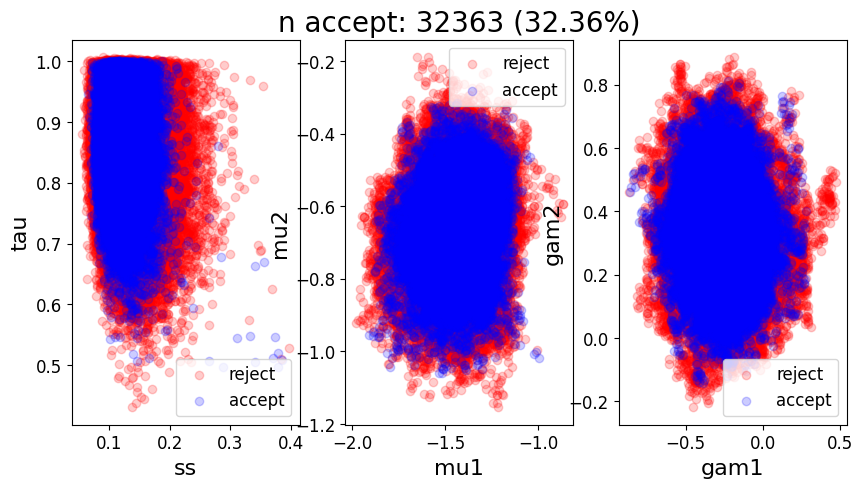
\includegraphics[width=.8\linewidth]{"./hmc_dist.png"}
  \caption{\label{fig:hmc_dist} Bivariate distributions for samples drawn from the HMC algorithm}
\end{figure}

\begin{figure}[H]
  \centering
  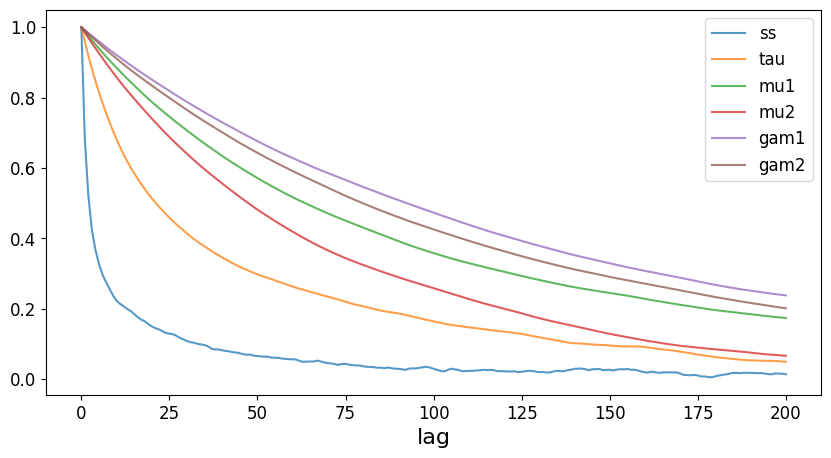
\includegraphics[width=.8\linewidth]{"./hmc_acorr.png"}
  \caption{\label{fig:hmc_acorr} Autocorrelation for each parameter value drawn from the HMC algorithm}
\end{figure}

\begin{figure}[H]
  \centering
  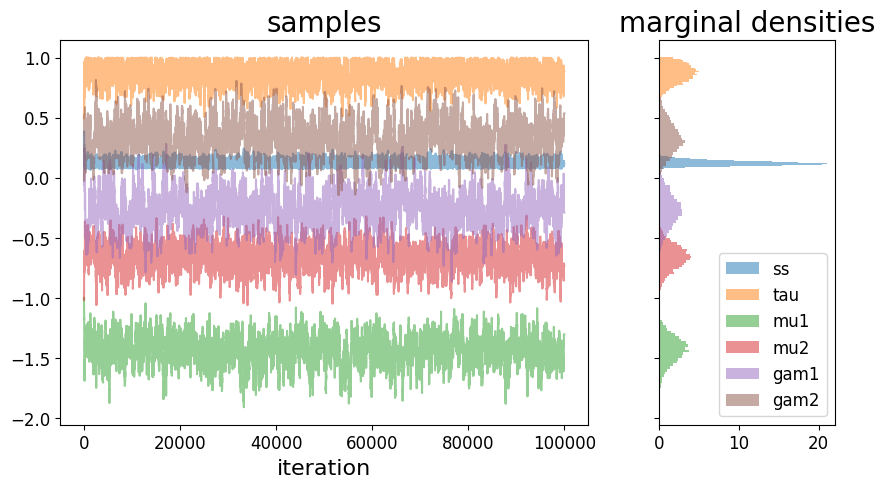
\includegraphics[width=.8\linewidth]{"./hmc_marg.png"}
  \caption{\label{fig:hmc_marg} Evolution of the HMC algorithm and accumulated marginal distributions}
\end{figure}

\begin{table}[H]
  \begin{center}
    \begin{tabular}{lrrrrrr}
      &$\sigma^2$ & $\tau$ & $\mu_1$ & $\mu_2$ & $\gamma_1$ & $\gamma_2$ \\
      \midrule
      mean   &  0.120568 &  0.863886 & -1.433177 & -0.662749 & -0.268818 &  0.329712 \\
      var    &  0.000406 &  0.006003 &  0.013752 &  0.011229 &  0.021705 &  0.019261 \\
      median &  0.118352 &  0.869840 & -1.427280 & -0.659320 & -0.269174 &  0.323608 \\
      p0     &  0.065007 &  0.495930 & -1.908123 & -1.059554 & -0.862452 & -0.143813 \\
      p10    &  0.096797 &  0.760097 & -1.585403 & -0.799194 & -0.457929 &  0.154746 \\
      p25    &  0.106273 &  0.810910 & -1.507754 & -0.730388 & -0.364532 &  0.237090 \\
      p50    &  0.118352 &  0.869840 & -1.427280 & -0.659320 & -0.269174 &  0.323608 \\
      p75    &  0.132432 &  0.924183 & -1.352740 & -0.591091 & -0.174501 &  0.421964 \\
      p90    &  0.147103 &  0.963355 & -1.289032 & -0.530516 & -0.082192 &  0.517047 \\
      p100   &  0.385267 &  1.002555 & -0.997103 & -0.314419 &  0.282297 &  0.813231 \\
      \bottomrule
      \end{tabular}
  \end{center}
  \caption{\label{tab:hmc_univar} Univariate statistics from samples drawn from the HMC algorithm}
\end{table}

\begin{table}[H]
  \begin{center}
    \begin{tabular}{lrrrrrr}
      {} & $\sigma^2$ & $\tau$ & $\mu_1$ & $\mu_2$ & $\gamma_1$ & $\gamma_2$ \\
      \midrule
      $\sigma^2$   &  0.000406 & -0.000174 & -0.000109 & -0.000148 & -0.000030 &  0.000069 \\
      $\tau$  & -0.000174 &  0.006003 &  0.004706 &  0.003352 & -0.000798 &  0.000399 \\
      $\mu_1$  & -0.000109 &  0.004706 &  0.013752 &  0.001797 & -0.006199 &  0.001104 \\
      $\mu_2$  & -0.000148 &  0.003352 &  0.001797 &  0.011230 & -0.000166 & -0.005065 \\
      $\gamma_1$ & -0.000030 & -0.000798 & -0.006199 & -0.000166 &  0.021706 & -0.000984 \\
      $\gamma_2$ &  0.000069 &  0.000399 &  0.001104 & -0.005065 & -0.000984 &  0.019261 \\
      \bottomrule
      \end{tabular}
  \end{center}
  \caption{\label{tab:hmc_covar} Covariance between parameters from distributions drawn from the HMC algorithm}
\end{table}


% -------------------------------------------------------------------------------
% IMPORTANCE SAMPLING
\section{Importance sampling}
\subsection{Implementation}
In this section I implement importance sampling with normalization to estimate sample statistics from my posterior distribution of model parameters. This technique allows me to draw samples, $\theta_i$, from a trial distribution, $q(\theta)$, and weight those samples with weights $w_i$ to achieve these sample statistics. Normalization allows me to use this approach for a function proportional to my target distribution, $f(\theta)$, up to an integrating constant (i.e., $p(\theta \mid Y) \propto\; f(\theta))$.

We show in class that importance sampling with normalization yields weighted samples where the sum of those weighted samples is a biased estimate of the expectation of the target distribution. Further, we show that the sum of any function of those weighted samples is a biased estimates of the expectation of that function, under the target distribution.

Like Metropolis-Hasting, implementing this method requires selecting a target distribution. A naive approach to this could involve selecting a multivariate t-distribution with support covering that of the target distribution. The t-distribution with a low degree of freedom is a good choice for such a candidate because of its wider tails, allowing samples to be drawn with higher likelihood over a wider range. 

In this instance, however, I notice that I can implement a form of two-stage Importance Sampling where I can construct a candidate distribution closer to my target distribution. This is desireable because drawing samples closer to my target distribution can increase the efficiency of my algorithm.

I observe that my target distribution can be re-written as the outcome of sequential posterior distribution calculations. Specifically
\begin{align}
  p(\theta \mid Y) = p(\sigma^2, \tau, \mu, \gamma \mid Y) &\propto\; p(\sigma^2) p(\tau) p(\mu) p(\gamma)\times \prod_{i\in g_1, g_2, g_3, g_4} L(y_i \mid \sigma^2, \tau, \mu, \gamma)\\
  &\propto\; (\sigma^2) p(\mu) p(\gamma) \times \prod_{i\in g_1, g_2} L(y_i \mid \sigma^2, \mu, \gamma) \times p(\tau) \times \prod_{i\in g_3, g_4} L(y_i \mid \sigma^2, \tau, \mu, \gamma)\\
  &\propto\; p(\sigma^2, \mu, \gamma \mid Y_{1,2}) \times p(\tau) \times \prod_{i\in g_3, g_4} L(y_i \mid \sigma^2, \tau, \mu, \gamma)
\end{align}
I next observe that the posterior, $p(\sigma^2, \mu, \gamma \mid Y_{1,2})$ can be computed in closed form.
\begin{align}
  q(\sigma^2, \mu, \gamma \mid Y_{1,2}) &= q(\mu, \gamma \mid Y_{1,2}) \times q(\sigma^2 \mid \mu, \gamma, Y_{1,2}) \textrm{, where}\\
  q(\mu, \gamma \mid Y_{1,2}) &\sim t_4\left(\mu= \left(\begin{matrix*}
    \overline{Y_1}\\ \overline{Y_2} \end{matrix*}\right), \Sigma=\frac{\sum_{i\in g_1}\lVert y_i - \overline{Y_1} \rVert^2 + \sum_{i \in g_2}\lVert y_i - \overline{Y_2}\rVert^2}{\nu}\left(\begin{matrix*}
      n_1^{-1} & 0 & 0 & 0 \\ 0 & n_1^{-1} & 0 & 0 \\ 0 & 0 & n_2^{-1} & 0 \\ 0 & 0 & 0 & n_2^{-1}
    \end{matrix*}\right), \nu=2(n_1 + n_2) - 4\right)\\
  q(\sigma^2 \mid \mu, \gamma, Y_{1,2}) &\sim InvGamma\left(\alpha=n_1 + n_2, \beta = \frac{1}{2}\sum_{i\in g_1}\lVert y_i - \mu\rVert^2 + \sum_{i\in g_2}\lVert y_i - \gamma\rVert^2\right)
\end{align}
Lastly, I note that for a trial density $q(\theta) := p(\sigma^2, \mu, \gamma \mid Y_{1,2}) \times p(\tau)$, I can estimate unnormalized sample weights in a straightforward manner. Notably
\begin{align}
  w_i := \frac{p(\theta_i)}{q(\theta_i)} = \frac{p(\sigma^2, \tau, \mu, \gamma \mid Y)}{p(\sigma^2, \mu, \gamma \mid Y_{1,2}) \times p(\tau)} \propto\; \frac{p(\sigma^2, \mu, \gamma \mid Y_{1,2}) \times p(\tau) \times \prod_{i\in g_3, g_4} L(y_i \mid \sigma^2, \tau, \mu, \gamma)}{p(\sigma^2, \mu, \gamma \mid Y_{1,2})\times p(\tau)} = \prod_{i\in g_3, g_4} L(y_i \mid \sigma^2, \tau, \mu, \gamma) =: u_i
\end{align}
Using the normalization method proved in class lecture, it follows cleanly that $w_i = u_i / \sum_{j=1}^nu_j$. I present all derivations of the distributions above in Appendix \ref{sec:a_is} and I present my sampling method below in Algorithm \ref{alg:is}.

\begin{algorithm}[H]
\caption{\label{alg:is} Importance sampling}
  \begin{algorithmic}
    \State $\theta_0 \longleftarrow$  Initialize
    \For{t=1, \dots, T}
      \State $\theta_i[\mu, \gamma] \sim q(\mu, \gamma \mid Y_{1,2})$
      \State $\theta_i[\sigma^2] \sim q(\sigma^2 \mid \theta_i[\mu, \gamma], Y_{1,2})$
      \State $\theta_i[\tau] \sim p(\tau)$
      \State $u_i = f(\theta_i \mid Y) / q(\theta_i)$  \Comment{$f(\theta_i \mid Y) \propto p(\theta_i \mid Y)$}
    \EndFor
    \State $\textbf{w} = \textbf{u} / \sum_{j=1}^n u_j$ \Comment{$\textbf{u}$ is a vector of all $u_i$}
    \State $\hat{\boldsymbol{\theta}} = \boldsymbol{\theta}*\textbf{w}$ \Comment{element-wise product; $\boldsymbol{\theta}$ is a vector of all $\theta_i$} 
  \end{algorithmic}
\end{algorithm}

Unlike the Metropolis-Hastings, Gibbs Sampling, and Hamiltonian Monte Carlo sampling approaches that enable me to draw samples from my target distribution, Importance Sampling only enables me to estimate sample statistics from my target distribution, in the form
\begin{align}
  \sum_i^n\theta_i w_i &\approxeq E\left[ \theta\right]\\
  \sum_i^nh(\theta_i)w_i &\approxeq E\left[ h(\theta) \right]
\end{align}
Below I list the statistics that I consider, and the functions, $h(\theta)$, I use to calculate each.
\begin{itemize}
  \item Expectation: $h(\theta[i]) = \theta[i]$
  \item Variance: $h(\theta[i]) = \left(\theta[i] - \frac{1}{n}\sum_k^n\theta[i]_k\right)^2$
  \item Covariance: $h(\theta[i], \theta[j]) = \left(\theta[i] - \frac{1}{n}\sum_k^n\theta[i]_k\right)\left(\theta[j] - \frac{1}{n}\sum_k^n\theta[j]_k\right)$
  \item $P(\theta[i] \in A)$: $h(\theta[i]) = \mathcal{I}\{ \theta[i] \in A \}$
\end{itemize}

\subsection{Results}
Below I present results from running the Importance Sampling algorithm for $T=1,000,000$ iterations. Table \ref{tab:is_univar} includes my estimates of mean and variance, Table \ref{tab:is_covar} includes my estimates of covariance, and Figure \ref{fig:is_marg} presents a histogram representation of the samples drawn for my target distribution. I observe close alignment between these statistics and those calculated using the other approaches.

\begin{table}[H]
  \begin{center}
    \begin{tabular}{lrrrrrr}
      &$\sigma^2$ & $\tau$ & $\mu_1$ & $\mu_2$ & $\gamma_1$ & $\gamma_2$ \\
      \midrule
      mean &  0.126739 &  0.856402 & -1.436720 & -0.662003 & -0.270092 &  0.323731 \\
      var  &  0.004417 &  0.134849 &  0.017131 &  0.071006 &  0.029327 &  0.044514 \\
      \bottomrule
      \end{tabular}
  \end{center}
  \caption{\label{tab:is_univar} Univariate statistics from samples drawn using Importance Sampling}
\end{table}

\begin{table}[H]
  \begin{center}
    \begin{tabular}{lrrrrrr}
      {} & $\sigma^2$ & $\tau$ & $\mu_1$ & $\mu_2$ & $\gamma_1$ & $\gamma_2$ \\
      \midrule
      $\sigma^2$&   0.004417 &  0.021157 & -0.002167 & -0.014401 & -0.004432 & -0.008876 \\\
      $\tau$  &    0.021157 &  0.134849 & -0.007030 & -0.081933 & -0.026803 & -0.051698 \\
      $\mu_1$  &  -0.002167 & -0.007030 &  0.017131 &  0.010279 & -0.004102 &  0.005337 \\
      $\mu_2$  &  -0.014401 & -0.081933 &  0.010279 &  0.071006 &  0.016959 &  0.029509 \\
      $\gamma_1$&  -0.004432 & -0.026803 & -0.004102 &  0.016959 &  0.029327 &  0.011137 \\
      $\gamma_2$ &   -0.008876 & -0.051698 &  0.005337 &  0.029509 &  0.011137 &  0.044514 \\
      \bottomrule
      \end{tabular}
  \end{center}
  \caption{\label{tab:is_covar} Covariance between parameters from distributions drawn using Importance Sampling}
\end{table}

\begin{figure}[H]
  \centering
  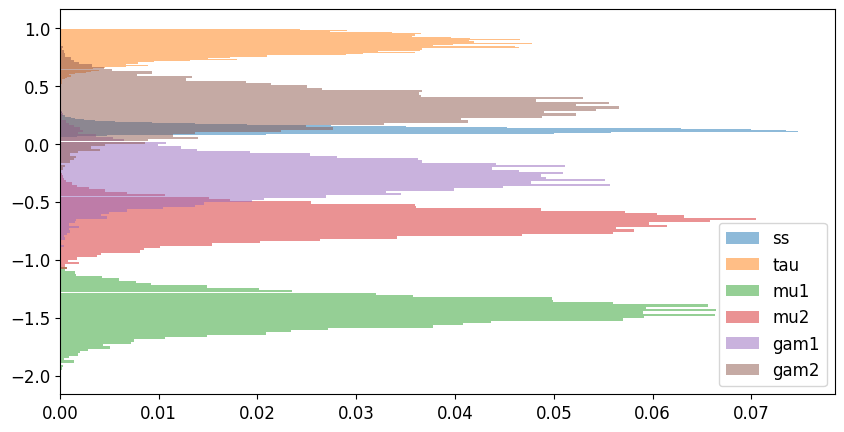
\includegraphics[width=.8\linewidth]{"./is_marg.png"}
  \caption{\label{fig:is_marg} Histogram of weighted samples drawn using Importance Sampling}
\end{figure}

I also include Figure \ref{fig:is_c_dist} and Figure \ref{fig:is_c_marg} revealing the draws from my candidate distribution, $q(\theta)$. I observe that these proposals track closely to the target distribution that I observe from my other sampling algorithms, validating this candidate distribution.

\begin{figure}[H]
  \centering
  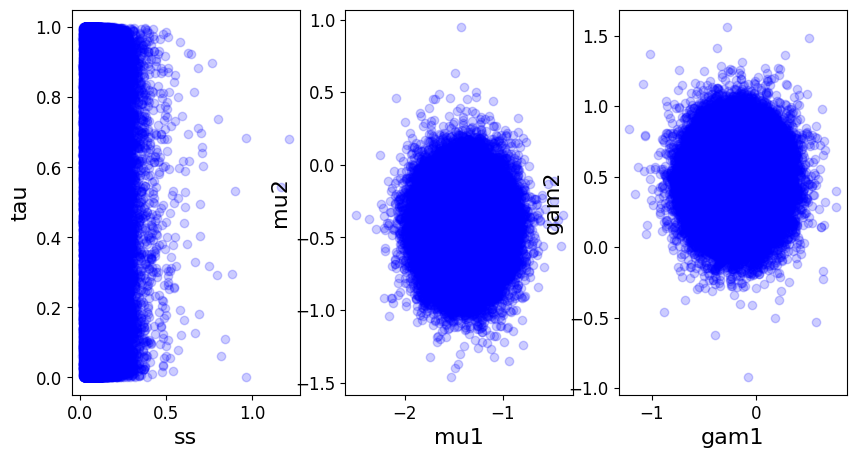
\includegraphics[width=.8\linewidth]{"./is_c_dist.png"}
  \caption{\label{fig:is_c_dist} Bivariate distributions for candidate samples (before weighting) drawn using Importance Sampling}
\end{figure}

\begin{figure}[H]
  \centering
  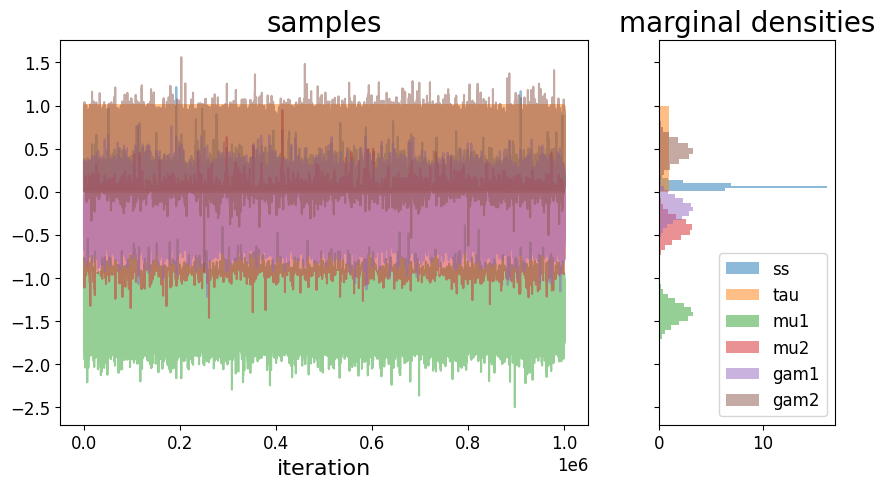
\includegraphics[width=.8\linewidth]{"./is_c_marg.png"}
  \caption{\label{fig:is_c_marg} Sample points and accumulated marginal distributions drawn (before weighting) using Importance Sampling}
\end{figure}







% ------------------------------------------------------------------------------------------------
\section{Discussion and conclusion}
To conclude this project, I compare the results from the four implemented methods to confirm my findings about the posterior distribution motivating this work. 

In Table \ref{tab:c_theta} I present the summary statistics for each parameter value using each approach. Overall, I observe that all methods agree closely (down to 2 decimal points) on the mean of each parameter value. Overall, I see agreement across other statistics like variance, median, and range. I observe that for $\tau$, Importance Sampling yields a variance two orders of magnitude higher, although this might be expected given how I constructed my candidate distribution for Importance Sampling (I simply assumed a uniform distribution on $\tau$). Also noteworthy is that Hamiltonian Monte Carlo reaches narrower limits for $\gamma_1$ and $\gamma_2$ than the other methods by about $0.1 - 0.3$. I suspect that the HMC algorithm could be tuned, in particular the $M$ matrix, in order to address this potential concern. 

In Table \ref{tab:c_overall} I present overall descriptive statistics for each of the approaches, including the achieved acceptance probabilities, a qualitative summary of their autocorrelation, and runtime to generate $100,000$ iterations. As I report, Gibbs sampling performs best across these parameters, with an acceptance rate of 1 and extremely low autocorrelation. My Hamiltonian Monte Carlo method performs roughly as well as the Metropolis Hastings algorithm, but at a much longer runtime.

In considering the scalability of these algorithms, I note that new samples are generated in $\mathcal{O}(n)$ time for Metropolis-Hasting, Gibbs Sampling, and Importance Sampling, while new samples are generated in $\mathcal{O}(nL)$ time for Hamiltonian Monte Carlo. Gibbs Sampling and Importance Sampling, which simply draw from known probability distributions and avoid other steps like calculating the acceptance probability yield slightly better performance. 


\begin{table}[H]
  \begin{center}
    \begin{tabular}{llrrrrr}
 \textbf{Sampling approach} & $\theta[i]$ &  \textbf{Mean} & \textbf{Variance} & \textbf{Min} & \textbf{Median} & \textbf{Max} \\
      \midrule
           1. Metropolis-Hasting &  $\gamma_1$ & -0.267675 & 0.021396 & -1.003121 & -0.268092 &  0.511373 \\
               2. Gibbs Sampling &  $\gamma_1$ & -0.268469 & 0.023484 & -0.967721 & -0.268257 &  0.565895 \\
      3. Hamiltonian Monte Carlo &  $\gamma_1$ & -0.268818 & 0.021705 & -0.862452 & -0.269174 &  0.282297 \\
          4. Importance Sampling &  $\gamma_1$ & -0.262994 & 0.028709 &       NaN &       NaN &       NaN \\
          \midrule
           1. Metropolis-Hasting &  $\gamma_2$ &  0.321261 & 0.021500 & -0.253334 &  0.320839 &  0.908794 \\
               2. Gibbs Sampling &  $\gamma_2$ &  0.321858 & 0.023579 & -0.447171 &  0.321986 &  1.055153 \\
      3. Hamiltonian Monte Carlo &  $\gamma_2$ &  0.329712 & 0.019261 & -0.143813 &  0.323608 &  0.813231 \\
          4. Importance Sampling &  $\gamma_2$ &  0.322258 & 0.044306 &       NaN &       NaN &       NaN \\
\midrule
           1. Metropolis-Hasting &   $\mu_1$ & -1.433174 & 0.014490 & -1.976549 & -1.428254 & -0.988145 \\
               2. Gibbs Sampling &   $\mu_1$ & -1.437019 & 0.015991 & -2.031535 & -1.432194 & -0.924040 \\
      3. Hamiltonian Monte Carlo &   $\mu_1$ & -1.433177 & 0.013752 & -1.908123 & -1.427280 & -0.997103 \\
          4. Importance Sampling &   $\mu_1$ & -1.438831 & 0.018104 &       NaN &       NaN &       NaN \\
\midrule
           1. Metropolis-Hasting &   $\mu_2$ & -0.660694 & 0.012879 & -1.293310 & -0.656396 & -0.248247 \\
               2. Gibbs Sampling &   $\mu_2$ & -0.663134 & 0.014178 & -1.258476 & -0.660151 & -0.043384 \\
      3. Hamiltonian Monte Carlo &   $\mu_2$ & -0.662749 & 0.011229 & -1.059554 & -0.659320 & -0.314419 \\
          4. Importance Sampling &   $\mu_2$ & -0.663804 & 0.072521 &       NaN &       NaN &       NaN \\
\midrule
           1. Metropolis-Hasting &    $\sigma^2$ &  0.114662 & 0.000567 &  0.060772 &  0.112433 &  0.250000 \\
               2. Gibbs Sampling &    $\sigma^2$ &  0.127170 & 0.000826 &  0.050965 &  0.123141 &  0.707467 \\
      3. Hamiltonian Monte Carlo &    $\sigma^2$ &  0.120568 & 0.000406 &  0.065007 &  0.118352 &  0.385267 \\
          4. Importance Sampling &    $\sigma^2$ &  0.127053 & 0.004413 &       NaN &       NaN &       NaN \\
\midrule
           1. Metropolis-Hasting &   $\tau$ &  0.861065 & 0.006893 &  0.448267 &  0.867656 &  0.999952 \\
               2. Gibbs Sampling &   $\tau$ &  0.856402 & 0.007462 &  0.353123 &  0.864109 &  0.999996 \\
      3. Hamiltonian Monte Carlo &   $\tau$ &  0.863886 & 0.006003 &  0.495930 &  0.869840 &  1.002555 \\
          4. Importance Sampling &   $\tau$ &  0.850954 & 0.131497 &       NaN &       NaN &       NaN \\
      \bottomrule
      \end{tabular}
\end{center}
  \caption{\label{tab:c_theta} Comparisson of performance metrics across algorithms}
\end{table}


\begin{table}[H]
  \begin{center}
\begin{tabular}{lrrr}
  \textbf{Sampling approach} &  \textbf{Acceptance rate} & \textbf{Autocorrelation} &  \textbf{100k iter runtime} \\
  \midrule
       1. Metropolis-Hasting &  0.35608 &  high & 03:32 \\
           2. Gibbs Sampling &  1.00000 &   low & 01:37 \\
  3. Hamiltonian Monte Carlo &  0.32363 &   low & 30.53 \\
      4. Importance Sampling &      - &  - & 01:08 \\
  \bottomrule
  \end{tabular}
\end{center}
  \caption{\label{tab:c_overall} Comparisson of performance metrics across algorithms}
\end{table}









%------------------------------------------------------------------------
% REFERENCES
{\small
\bibliographystyle{ieee}
\bibliography{egbib}
}

%------------------------------------------------------------------------
% Appendix
\section{Appendix}
\subsection{Derivation of the posterior, $p(\theta \mid Y)$}
\label{sec:a_post}
\subsubsection{Provided models for gene expression}
\begin{align*}
  (y_i | g_i = 1) &\sim N(\mu, \sigma^2 I)\\
  (y_i | g_i = 2) &\sim N(\gamma, \sigma^2 I)\\
  (y_i | g_i = 3) &\sim N(\frac{1}{2}(\mu + \gamma), \sigma^2 I)\\
  (y_i | g_i = 4) &\sim N(\tau\mu + (1-\tau)\gamma, \sigma^2 I)
\end{align*}
\subsubsection{Provided priors for gene expression models}
\begin{align*}
  \theta &= (\sigma^2, \tau, \mu_1, \mu_2, \gamma_1, \gamma_2)\\
  p(\sigma^2) &\propto \frac{1}{\sigma^2}\\
  p(\tau) &\sim Unif[0, 1]\\
  p(\mu) &= p(\mu_1, \mu_2) \propto 1 \textrm{ (improper uniform)}\\
  p(\gamma) &= p(\gamma_1, \gamma_2) \propto 1 \textrm{ (improper uniform)}\\
\end{align*}
\subsubsection{Derivation of likelihood and posterior distribution}
\begin{align*}
  L(Y | \theta) =& \prod_{i=1}^n p(y_i | \theta) \textrm{, for } Y = (y_i, \dots, y_n)\\
  =& \prod_{i \in g_1} \frac{1}{\sqrt{2\pi}}((\sigma^2)^2)^{-\frac{1}{2}} \exp[-\frac{1}{2\sigma^2} (y_i - \mu)^T(y_i - \mu)] \times  
     \prod_{i\in g_2} \frac{1}{\sqrt{2\pi}}((\sigma^2)^2)^{-\frac{1}{2}} \exp[-\frac{1}{2\sigma^2} (y_i - \gamma)^T(y_i - \gamma)]\\
  &\times \prod_{i\in g_3} \frac{1}{\sqrt{2\pi}}((\sigma^2)^2)^{-\frac{1}{2}} \exp[-\frac{1}{2\sigma^2} (y_i - \frac{1}{2}(\mu +  
    \gamma))^T(y_i - \frac{1}{2}(\mu + \gamma))] \\
  &\times \prod_{i\in g_4} \frac{1}{\sqrt{2\pi}}((\sigma^2)^2)^{-\frac{1}{2}} \exp[-\frac{1}{2\sigma^2} (y_i - (\tau\mu + (1-\tau)\gamma))^T(y_i - (\tau\mu + (1-\tau)\gamma))] \\
  =& \left(\frac{1}{\sigma^2\sqrt{2\pi}}\right)^n \exp[-\frac{1}{2\sigma^2}(\sum_{i\in g_1}(y_i - \mu)^T(y_i -   \mu) + \sum_{i\in g_2}(y_i - \gamma)^T(y_i - \gamma)\\
  &+ \sum_{i\in g_3}(y_i - \frac{1}{2}(\mu +  
  \gamma))^T(y_i - \frac{1}{2}(\mu + \gamma)) + \sum_{i\in g_4}(y_i - (\tau\mu + (1-\tau)\gamma))^T(y_i - (\tau\mu + (1-\tau)\gamma)))]\\\\
  p(\theta | Y) \propto&\; p(\theta) L(Y | \theta)
\end{align*}

\subsection{Metropolis Hasting}
\label{sec:a_mh}
\subsubsection{Results of hyperparameter tuning}
\begin{table}[H]
  \begin{center}
\begin{tabular}{rrrrr}
  $\nu_{\sigma^2}$ & $\nu_\tau$ & $\nu_{\mu, \gamma}$ & \textbf{Acceptance rate} & \textbf{Max lag $\leq 0.2$} \\
  \midrule
  0.005 &    0.01 &   0.01 &         0.285000 &           36.0 \\
  0.001 &    0.01 &   0.01 &         0.323333 &           96.0 \\
  0.050 &    0.01 &   0.01 &         0.240000 &           34.0 \\
  0.005 &    0.05 &   0.01 &         0.188333 &           40.0 \\
  0.001 &    0.05 &   0.01 &         0.261667 &          111.0 \\
  0.050 &    0.05 &   0.01 &         0.181667 &           44.0 \\
  0.005 &    0.10 &   0.01 &         0.193333 &          106.0 \\
  0.001 &    0.10 &   0.01 &         0.205000 &          147.0 \\
  0.050 &    0.10 &   0.01 &         0.156667 &           54.0 \\
  0.005 &    0.01 &   0.05 &         0.141667 &          108.0 \\
  0.001 &    0.01 &   0.05 &         0.141667 &           81.0 \\
  0.050 &    0.01 &   0.05 &         0.090000 &           70.0 \\
  0.005 &    0.05 &   0.05 &         0.096667 &          101.0 \\
  0.001 &    0.05 &   0.05 &         0.133333 &          142.0 \\
  0.050 &    0.05 &   0.05 &         0.041667 &           79.0 \\
  0.005 &    0.10 &   0.05 &         0.111667 &           56.0 \\
  0.001 &    0.10 &   0.05 &         0.096667 &          153.0 \\
  0.050 &    0.10 &   0.05 &         0.031667 &           86.0 \\
  0.005 &    0.01 &   0.10 &         0.063333 &           94.0 \\
  0.001 &    0.01 &   0.10 &         0.091667 &          122.0 \\
  0.050 &    0.01 &   0.10 &         0.040000 &           51.0 \\
  0.005 &    0.05 &   0.10 &         0.046667 &          129.0 \\
  0.001 &    0.05 &   0.10 &         0.070000 &          119.0 \\
  0.050 &    0.05 &   0.10 &         0.045000 &           93.0 \\
  0.005 &    0.10 &   0.10 &         0.053333 &          139.0 \\
  0.001 &    0.10 &   0.10 &         0.033333 &          169.0 \\
  0.050 &    0.10 &   0.10 &         0.040000 &           58.0 \\
 \bottomrule
 \end{tabular}
\end{center}
 \caption{\label{tab:mh_gridsearch} Grid search across candidate distribution variances}
\end{table}


\subsection{Gibbs sampling}
\label{sec:a_gibbs}
\subsubsection{Derivation of $p(\tau \mid \sigma^2, \mu, \gamma, Y)$}
\begin{align*}
  p(\tau | Y, \theta[-\tau]) &\propto p(\theta)L(Y | \theta)\\  
  & \propto p(\tau)\prod_{i\in g_4} \frac{1}{\sigma^2\sqrt{2\pi}} \exp[-\frac{1}{2\sigma^2} (y_i - (\tau\mu + (1-\tau)\gamma))^T(y_i - (\tau\mu + (1-\tau)\gamma))]\\
  &\propto \exp[-\frac{1}{2\sigma^2}\sum_{i\in g_4}(y_i - (\tau\mu + (1-\tau)\gamma))^T(y_i - (\tau\mu + (1-\tau)\gamma))] \textrm{, for } \tau \in [0,1]\\
  &\propto \exp[-\frac{1}{2\sigma^2}\sum_{i\in g_4}(y_i^Ty_i - 2y_i^T(\tau\mu + (1-\tau)\gamma) + (\tau\mu + (1-\tau)\gamma)^T(\tau\mu + (1-\tau)\gamma))] \textrm{, for } \tau \in [0,1]\\
  &\propto \exp[-\frac{1}{2\sigma^2}\sum_{i\in g_4} \tau^2(\mu^T\mu - 2\mu^T\gamma + \gamma^T\gamma) - 2\tau(y_i^T\mu - y_i^T\gamma - \mu^T\gamma + \gamma^T\gamma)]\textrm{, for } \tau \in [0,1]\\
  &\propto \exp[-\frac{1}{2\sigma^2}(n_4 \tau^2(\mu - \gamma)^T(\mu - \gamma) - 2\tau(\mu - \gamma)^T[\sum_{i\in g_4}(y_i - \gamma) \textrm{, for } \tau \in [0,1]\\
  &\propto \exp\left[-\frac{1}{2}*\frac{n_4(\mu - \gamma)^T(\mu - \gamma)}{\sigma^2}\left(\tau - \frac{(\mu - \gamma)^T(\sum_{i\in g_4}(y_i - \gamma))}{n_4(\mu - \gamma)^T(\mu - \gamma)}\right)^2\right] \textrm{, for } \tau \in [0,1]\\
  &\sim Norm\left(\mu=\frac{(\mu - \gamma)^T(\sum_{i\in g_4}(y_i - \gamma))}{n_4(\mu - \gamma)^T(\mu - \gamma)}, \sigma^2=\frac{\sigma^2}{n_4(\mu - \gamma)^T(\mu - \gamma)}\right) \textrm{, truncated to } [0,1]
\end{align*}

\subsubsection*{Derivation of $p(\sigma^2 \mid \tau, \mu, \gamma, Y)$}
\begin{align*}
  p(\sigma^2 \mid Y, \theta[-\sigma^2]) \propto& p(\theta)L(Y | \theta) \propto p(\sigma^2) \prod_{i=1}^n p(y_i | \theta)\\
  \propto& \frac{1}{\sigma^2} * \left(\frac{1}{\sigma^2}\right)^n \exp\left[-\frac{1}{2\sigma^2}M\right] \textrm{, where } M = \\
  &\;\;\; \sum_{i\in g_1}(y_i - \mu)^T(y_i -   \mu) + \sum_{i\in g_2}(y_i - \gamma)^T(y_i - \gamma)+ \sum_{i\in g_3}(y_i - \frac{1}{2}(\mu +  
  \gamma))^T(y_i - \frac{1}{2}(\mu + \gamma))\\
  &\;\;\; + \sum_{i\in g_4}(y_i - (\tau\mu + (1-\tau)\gamma))^T(y_i - (\tau\mu + (1-\tau)\gamma))\\
  \propto& (\sigma^2)^{-n - 1}\exp\left[-\frac{M}{2}\frac{1}{\sigma^2}\right]\\
  \sim& InvGamma\left(\alpha=n, \beta = \frac{M}{2}\right)
\end{align*}

\subsubsection{Derivation of $p(\mu \mid \sigma^2, \tau, \gamma, Y)$}
\begin{align*}
  p(\mu | Y, \theta[-\mu]) \propto& p(\theta)L(Y | \theta)\\
  \propto& \prod_{i \in g_1} \frac{1}{\sigma^2\sqrt{2\pi}} \exp[-\frac{1}{2\sigma^2} (y_i - \mu)^T(y_i - \mu)]
    \times \prod_{i\in g_3} \frac{1}{\sigma^2\sqrt{2\pi}} \exp[-\frac{1}{2\sigma^2} (y_i - \frac{1}{2}(\mu +  
    \gamma))^T(y_i - \frac{1}{2}(\mu + \gamma))] \\
  &\times \prod_{i\in g_4} \frac{1}{\sigma^2\sqrt{2\pi}} \exp[-\frac{1}{2\sigma^2} (y_i - (\tau\mu + (1-\tau)\gamma))^T(y_i - (\tau\mu + (1-\tau)\gamma))]\\
  \propto& \exp[-\frac{1}{2\sigma^2}(n_1\mu^T\mu - 2\mu^T\left(\sum_{i\in g_1}y_i\right) - \mu^T\left(\sum_{i\in g_3}y_i\right) + \frac{n_3}{4}\mu^T\mu + \frac{n_3}{2}\mu^T\gamma\\
  &-2\tau\mu^T\left(\sum_{i\in g_4}y_i\right) + \tau^2n_4\mu^T\mu + 2\tau(1 - \tau)n_4\mu^T\gamma )]\\
  \propto& \exp\left[-\frac{1}{2\sigma^2}(n_1 + \frac{n_3}{4} + n_4\tau^2)\left(\mu^T\mu - 2\mu^T\frac{\sum_{i \in g_1}y_i + \frac{1}{2}\sum_{i\in g_3}y_i + \tau\sum_{i\in g_4}y_i - (\frac{n_3}{4} + n_4\tau(1 - \tau))\gamma}{n_1 + \frac{n_3}{4} + n_4\tau^2} \right)\right] \\
  \propto& \exp\left[-\frac{1}{2\phi^2}(\mu - \psi)^T(\mu - \psi)\right] \textrm{, where }\\
  &\;\;\; \psi = \frac{\sum_{i \in g_1}y_i + \frac{1}{2}\sum_{i\in g_3}y_i + \tau\sum_{i\in g_4}y_i - (\frac{n_3}{4} + n_4\tau(1 - \tau))\gamma}{n_1 + \frac{n_3}{4} + n_4\tau^2} \textrm{, } \phi^2 = \frac{\sigma^2}{n_1 + \frac{n_3}{4} + n_4\tau^2}\\
  \sim& N(\mu = \psi, \Sigma = \phi^2 I)
\end{align*}

\subsubsection{Derivation of $p(\gamma \mid \sigma^2, \tau, \mu, Y)$}
By symmetry with posterior conditional probability of $\mu$,
\begin{align*}
  p(\gamma | Y, \theta[-\gamma]) \sim& N(\mu = \psi', \Sigma = \phi'^2 I) \textrm{, where }\\
  &\;\;\; \psi' = \frac{\sum_{i \in g_2}y_i + \frac{1}{2}\sum_{i\in g_3}y_i + (1-\tau)\sum_{i\in g_4}y_i - (\frac{n_3}{4} + n_4\tau(1 - \tau))\mu}{n_2 + \frac{n_3}{4} + n_4(1-\tau)^2} \textrm{, } \phi'^2 = \frac{\sigma^2}{n_2 + \frac{n_3}{4} + n_4(1-\tau)^2}
\end{align*}


\subsection{Hamiltonian Monte Carlo}
\label{sec:a_hmc}
\subsubsection{Results of hyperparameter tuning}
\begin{table}[H]
  \begin{center}
\begin{tabular}{rrrr}
  \textbf{Scale of M} & \textbf{L} & $\epsilon$ & \textbf{Acceptance rate}\\
  \midrule
   1.0 &  5 &   0.0100 &            0.186 \\
   1.0 &  5 &   0.0010 &            0.410 \\
   1.0 &  5 &   0.0001 &            0.456 \\
   1.0 & 10 &   0.0100 &            0.028 \\
   1.0 & 10 &   0.0010 &            0.400 \\
   1.0 & 10 &   0.0001 &            0.386 \\
   1.0 & 20 &   0.0100 &            0.004 \\
   1.0 & 20 &   0.0010 &            0.338 \\
   1.0 & 20 &   0.0001 &            0.406 \\
   1.5 &  5 &   0.0100 &            0.272 \\
   1.5 &  5 &   0.0010 &            0.386 \\
   1.5 &  5 &   0.0001 &            0.462 \\
   1.5 & 10 &   0.0100 &            0.098 \\
   1.5 & 10 &   0.0010 &            0.484 \\
   1.5 & 10 &   0.0001 &            0.370 \\
   1.5 & 20 &   0.0100 &            0.020 \\
   1.5 & 20 &   0.0010 &            0.412 \\
   1.5 & 20 &   0.0001 &            0.460 \\
   2.0 &  5 &   0.0100 &            0.272 \\
   2.0 &  5 &   0.0010 &            0.448 \\
   2.0 &  5 &   0.0001 &            0.418 \\
   2.0 & 10 &   0.0100 &            0.242 \\
   2.0 & 10 &   0.0010 &            0.446 \\
   2.0 & 10 &   0.0001 &            0.398 \\
   2.0 & 20 &   0.0100 &            0.208 \\
   2.0 & 20 &   0.0010 &            0.436 \\
   2.0 & 20 &   0.0001 &            0.474 \\
 \bottomrule
 \end{tabular}
\end{center}
 \caption{\label{tab:hmc_gridsearch} Grid search across candidate distribution variances}
\end{table}




\subsection{Importance sampling}
\label{sec:a_is}
\subsubsection{Derivation of $p(\sigma^2 \mid \mu, \gamma, Y_{1,2})$}
\begin{align*}
  q(\sigma^2 \mid \mu, \gamma, Y_{1,2})\propto&\;\; \frac{1}{\sigma^2} * \left(\frac{1}{\sigma^2}\right)^{n_1 + n_2} \exp\left[-\frac{1}{2\sigma^2}M\right] \textrm{, where } M = \sum_{i\in g_1}(y_i - \mu)^T(y_i -   \mu) + \sum_{i\in g_2}(y_i - \gamma)^T(y_i - \gamma)\\
  \propto&\;\; (\sigma^2)^{-n_1 - n_2 - 1}\exp\left[-\frac{M}{2}\frac{1}{\sigma^2}\right]\\
  \sim& InvGamma\left(\alpha=n_1 + n_2, \beta = \frac{M}{2}\right)
\end{align*}

\subsubsection{Derivation of $p(\mu, \gamma \mid Y_{1,2})$}
\begin{align*}
  q(\mu, \gamma \mid Y_{1,2}) =& \int_0^\infty q(\mu, \gamma, \sigma^2 \mid Y_{1,2})d\sigma^2\\
  \propto&\; \int_0^\infty\left(\frac{1}{\sigma^2}\right)^{n_1 + n_2 + n_3 + 1} \exp\left[-\frac{1}{2\sigma^2}(\sum_{i\in g_1} \lVert y_i - \mu\rVert^2 + \sum_{i\in g_2}\lVert y_i - \gamma \rVert^2\right]d\sigma^2\\
  \propto&\; \Gamma(n_1 + n_2) \left(-\frac{1}{2}  \sum_{i\in g_1} \lVert y_i - \mu\rVert^2 + \sum_{i\in g_2}\lVert y_i - \gamma \rVert^2\right)^{-(n_1 + n_2)}, \textrm{ where } \frac{\Gamma(\alpha)}{\beta^\alpha} = \int_0^\infty (\sigma^2)^{-\alpha - 1} \exp\left(\frac{\beta}{\sigma^2}\right)d\sigma^2\\
  \propto&\; (M + n_1\lVert \overline{Y_1} - \mu \rVert^2 + n_2\lVert \overline{Y_2} - \gamma \rVert^2)^{-(n_1 + n_2)}, \textrm{ where } M = \sum_{i\in g_1}\lVert y_i - \overline{Y_1} \rVert^2 + \sum_{i\in g_2}\lVert y_i - \overline{Y_2} \rVert^2\\
  \propto&\; \left(M + \left[\left(\begin{matrix}\mu\\ \gamma\end{matrix}\right) - \left(\begin{matrix*}\overline{Y_1}\\ \overline{Y_2}\end{matrix*}\right)\right]^T \left(\begin{matrix*} n_1 & 0 & 0 & 0 \\ 0 & n_1 & 0 & 0 \\ 0 & 0 & n_2 & 0 \\ 0 & 0 & 0 & n_2 \end{matrix*}\right) \left[\left(\begin{matrix}\mu\\ \gamma\end{matrix}\right) - \left(\begin{matrix*}\overline{Y_1}\\ \overline{Y_2}\end{matrix*}\right)\right]\right)^{-(n_1 + n_2)}\\
  \propto&\; \left(1 + \frac{1}{2(n_1 + n_2) - 4}\times\frac{2(n_1 + n_2) - 4}{M}\left[\left(\begin{matrix}\mu\\ \gamma\end{matrix}\right) - \left(\begin{matrix*}\overline{Y_1}\\ \overline{Y_2}\end{matrix*}\right)\right]^T \left(\begin{matrix*} n_1^{-1} & 0 & 0 & 0 \\ 0 & n_1^{-1} & 0 & 0 \\ 0 & 0 & n_2^{-1} & 0 \\ 0 & 0 & 0 & n_2^{-1} \end{matrix*}\right)^{-1} \left[\left(\begin{matrix}\mu\\ \gamma\end{matrix}\right) - \left(\begin{matrix*}\overline{Y_1}\\ \overline{Y_2}\end{matrix*}\right)\right]\right)^{-(n_1 + n_2)}\\
  \propto&\; \left[1 + \frac{1}{\nu}(x - \eta)^T\Sigma^{-1}(x - \eta)\right]^{-\frac{\nu + 4}{2}}, \textrm{where }\\
  &\;\; \nu=2(n_1 + n_2) + 4, \Sigma=\frac{M}{2(n_1 + n_2) - 4}\left(\begin{matrix*} n_1^{-1} & 0 & 0 & 0 \\ 0 & n_1^{-1} & 0 & 0 \\ 0 & 0 & n_2^{-1} & 0 \\ 0 & 0 & 0 & n_2^{-1} \end{matrix*}\right), \eta=\left(\begin{matrix*}\overline{Y_1}\\ \overline{Y_2}\end{matrix*}\right)\\
  q(\mu, \gamma \mid Y_{1,2}) &\sim t_4\left(\mu= \left(\begin{matrix*}
    \overline{Y_1}\\ \overline{Y_2} \end{matrix*}\right), \Sigma=\frac{\sum_{i\in g_1}\lVert y_i - \overline{Y_1} \rVert^2 + \sum_{i \in g_2}\lVert y_i - \overline{Y_2}\rVert^2}{\nu}\left(\begin{matrix*}
      n_1^{-1} & 0 & 0 & 0 \\ 0 & n_1^{-1} & 0 & 0 \\ 0 & 0 & n_2^{-1} & 0 \\ 0 & 0 & 0 & n_2^{-1}
    \end{matrix*}\right), \nu=2(n_1 + n_2) - 4 \right)
\end{align*}
\end{document}


